\documentclass[xcolor=table, 12pt, aspectratio=43,ignorenonframetext]{beamer}

%\documentclass{article}
%\usepackage{beamerarticle}

%\usepackage{arev}
\usepackage{amsmath,amssymb,amscd}
\usepackage{dsfont}
\usepackage{mathrsfs}
\usepackage{yfonts}
\usepackage{bm}
\usepackage{graphicx}
\usepackage{tabularx}
\usepackage{animate}
%\usepackage{ifthen}

%\usepackage{xeCJK}
%\usepackage{fontspec}
%\newfontfamily\cjkfont{PingFang SC}
%\setCJKmainfont{PingFang SC}
\newcolumntype{x}{>{\centering\arraybackslash}X}
\renewcommand{\arraystretch}{1.5}
\DeclareMathOperator{\img}{img}
\newcommand{\uone}{\text U(1)}

\usepackage{tikz}
	\usetikzlibrary{calc}
	\usetikzlibrary{arrows,shapes, positioning, matrix}
	\usetikzlibrary{decorations.markings}
	\tikzstyle arrowstyle=[scale=1]
  \tikzstyle string=[thick,postaction={decorate,decoration={markings,
      mark=at position .55 with {\arrow[arrowstyle]{stealth}}}}]

\usepackage{pgffor}
\newcommand{\cohosub}[1]{\scalebox{0.72}{\textswab{#1}}}
\newcommand{\cohosubsub}[1]{\scalebox{0.6}{\textswab{#1}}}
\newcommand{\coho}[1]{\textswab{#1}}


\mode<presentation>
{
  %\usetheme{Warsaw}
  % or ...
  %\useoutertheme{rectangle}
  \setbeamertemplate{frametitle}[default][center]
  \defbeamertemplate{itemize item}{flat}{\begin{pgfpicture}{-1ex}{0ex}{1ex}{2ex}
      \pgfpathcircle{\pgfpoint{0pt}{.6ex}}{0.6ex}
      \pgfusepath{fill}
    \end{pgfpicture}%
  }
  \defbeamertemplate{itemize subitem}{flat}{\footnotesize\raise0.5pt\hbox{\textbullet}}
  \defbeamertemplate{itemize subsubitem}{flat}{\footnotesize\raise0.5pt\hbox{\textbullet}}

  %\useinnertheme{circles}
  \setbeamertemplate{items}[flat]
  \setbeamertemplate{sections/subsections in toc}[circle]
  \setbeamertemplate{blocks}[rounded]
  \setbeamertemplate{title page}[default][colsep=-4bp,rounded=true]
  \setbeamertemplate{part page}[default][colsep=-4bp,rounded=true]
  \setbeamercovered{transparent}
  %\usecolortheme{spruce}
  %\definecolor{THU}{RGB}{116,61,130}
  \definecolor{mbg}{RGB}{0,0,160}
  \setbeamercolor*{palette primary}{fg=white,bg=mbg}
  \setbeamercolor*{titlelike}{parent=palette primary}
  \setbeamercolor*{structure}{fg=mbg}
  \setbeamercolor{frametitle}{fg=white,bg=mbg}
  % or whatever (possibly just delete it)
  \setbeamercolor{block title}{bg=mbg,fg=white}
  \setbeamercolor{block body}{bg=mbg!15}


  \addtobeamertemplate{navigation symbols}{}{ \hspace{1em}%
    \usebeamerfont{footline}%
    \insertframenumber / \inserttotalframenumber }
}


%\usepackage[english]{babel}
% or whatever

%\usepackage[latin1]{inputenc}
% or whatever

%\usepackage{times}
%\usepackage[T1]{fontenc}
% Or whatever. Note that the encoding and the font should match. If T1
% does not look nice, try deleting the line with the fontenc.

\title % (optional, use only with long paper titles)
{Lecture 1: SPT phases and cohomology theory}
\author[Y Qi] % (optional, use only with lots of authors)
{Yang~Qi}
% - Give the names in the same order as the appear in the paper.
% - Use the \inst{?} command only if the authors have different
%   affiliation.

\institute[Fudan] % (optional, but mostly needed)
{
Department of Physics, Fudan University.
}
% - Use the \inst command only if there are several affiliations.
% - Keep it simple, no one is interested in your street address.

%\date{2016 Annual Meeting of Fudan CFTPP} % (optional, should be abbreviation of conference name)
%{Fudan University, Oct 13 2015}
\date{Nov. 29-30, 2019}
% - Either use conference name or its abbreviation.
% - Not really informative to the audience, more for people (including
%   yourself) who are reading the slides online

%\subject{Theoretical Physics}
% This is only inserted into the PDF information catalog. Can be left
% out.



% If you have a file called "university-logo-filename.xxx", where xxx
% is a graphic format that can be processed by latex or pdflatex,
% resp., then you can add a logo as follows:

\pgfdeclareimage[height=1cm]{university-logo}{../resources/fudan}
\logo{\pgfuseimage{university-logo}}



% Delete this, if you do not want the table of contents to pop up at
% the beginning of each subsection:
\AtBeginSection[]
{
  \begin{frame}<beamer>{Outline}
			\tableofcontents[currentsection,currentsubsection]
  \end{frame}
}
%\AtBeginSubsection[]
%{
 % \begin{frame}<beamer>{Outline}
  %  \tableofcontents[currentsection,currentsubsection]
  %\end{frame}
%}


\begin{document}

\begin{frame}
  \titlepage
\end{frame}

\begin{frame}{Outline}
	%\begin{columns}
	%\column{.7\textwidth}
		\tableofcontents
  %\end{columns}
  % You might wish to add the option [pausesections]
\end{frame}

\section{Introduction: What are SPT states}

\begin{frame}
  \frametitle{Symmetry-Protected Topological (SPT) states}
\begin{itemize}
\item SPT: gapped topological phases beyond Landau paradiam.
\item Cannot be smoothly connected to a trivial state without closing gap or breaking symmetry.
\item Symmetry-protected gapless surface states.
\item Free-fermion states: topological insulators, topological superconductors.
\item Bosonic SPTs: Haldane chain, CZX/Levin-Gu state, etc.\\
\emph{Xie Chen, Zheng-Cheng Gu, Zheng-Xin Liu and Xiao-Gang Wen, Science 2012.}
\item Interacting fermionic SPTs.
\end{itemize}
\end{frame}

\begin{frame}
	\frametitle{Abelian-group classification}
	\begin{itemize}
		\item SPT phases and boundary anomalies are classified by Abelian groups ($\mathbb Z$ or $\mathbb Z_n$).
		\begin{itemize}
			\item Addition: stacking of phases/gapless boundaries.
			\item 0: The trivial phase/gapped boundary.
		\end{itemize}
		\item 2D Chern-insulators (Integer Quantum Hall):
		\begin{center}
				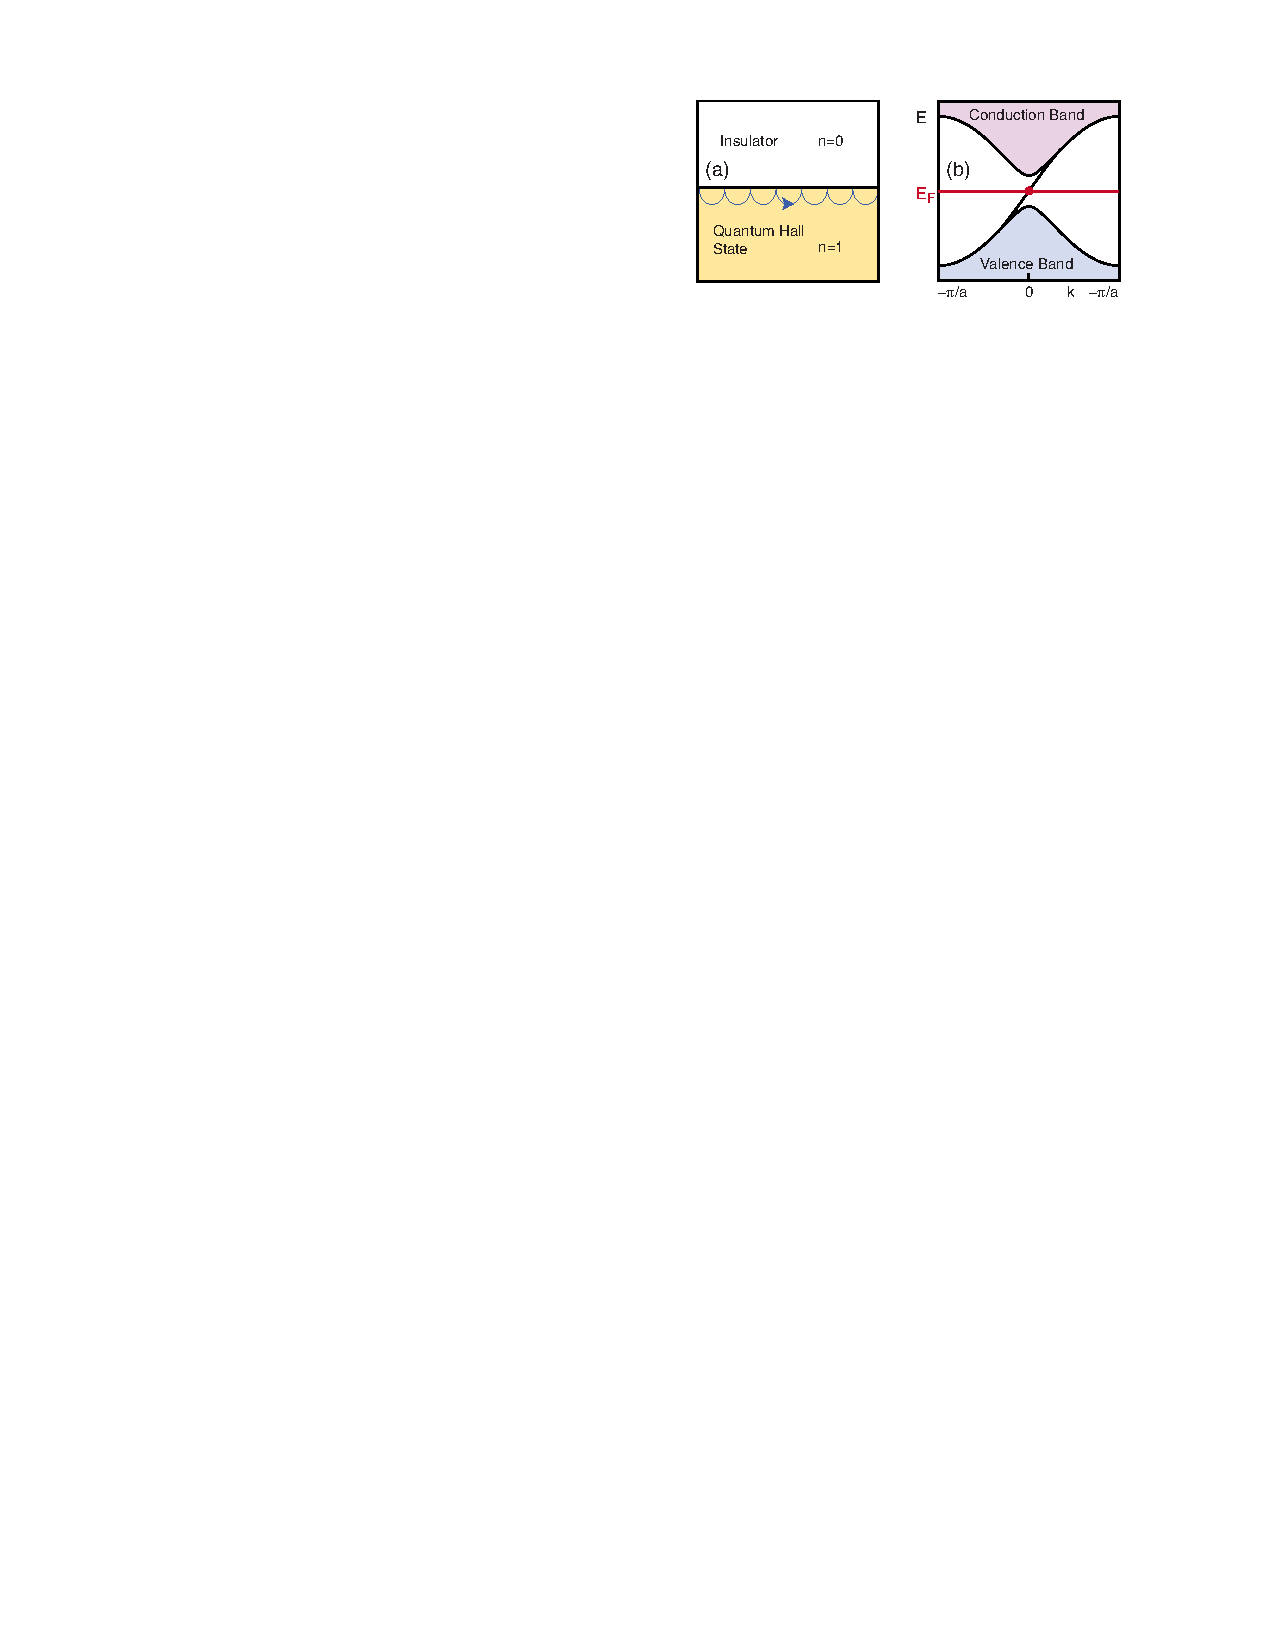
\includegraphics[width=8cm]{../spspt/qhe_edge}
		\end{center}
		Classified by $\mathbb Z$: $[n]+[m]=[n+m]$; $[n]+[-n] = 0$.
	\end{itemize}
\end{frame}

\begin{frame}
	\frametitle{Abelian-group classification}
	\begin{itemize}
		\item 3D Topological Insulators:
		\begin{center}
			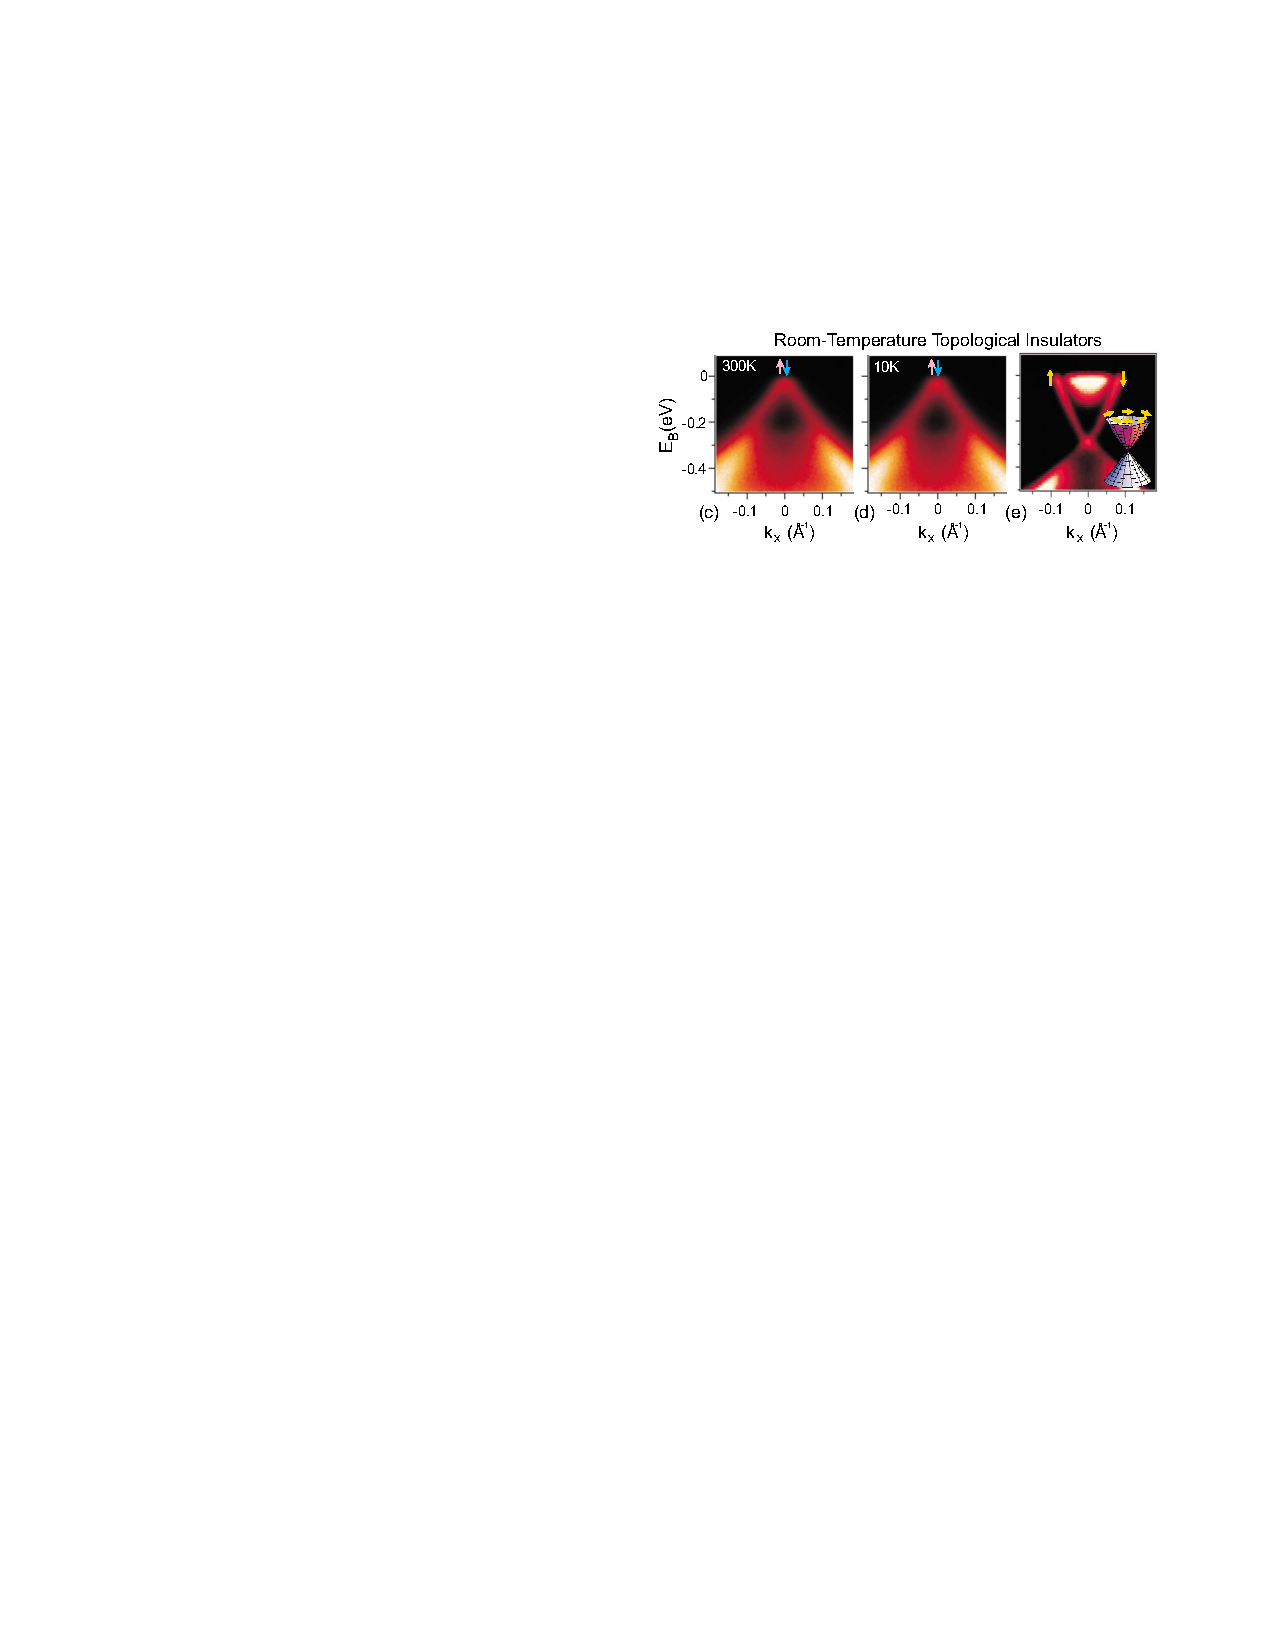
\includegraphics[width=8cm]{../spspt/ti_surface}
		\end{center}
		Classified by $\mathbb Z_2$: $[1]+[1] = 0$.
		\item 1D Haldane chain:
		\begin{center}
			
\includegraphics[width=6cm]{../dimer/weak3d_aklt_blue}
		\end{center}
		Classified by $\mathbb Z_2$: $[1]+[1] = 0$.
	\end{itemize}
\end{frame}

\section{Constructing an SPT state}

\begin{frame}
\frametitle{Group-cohomology model}
\begin{itemize}
\item Consider an onsite symmetry group $G$, $|G|<\infty$.
\item A space-time $\Delta$-lattice: $d+1$-simplexes (triangles, tetrahedra, etc).
\item Branching structure: an ordering $1>2>\cdots>N$; an orientation $i\rightarrow j$ if $i<j$. 
\item Hilbert space: $\otimes_i |g_i\rangle$, $g_i\in G$.
\item Symmetry transformation:
$g|g_i\rangle = |gg_i\rangle$.
\end{itemize}
\begin{center}
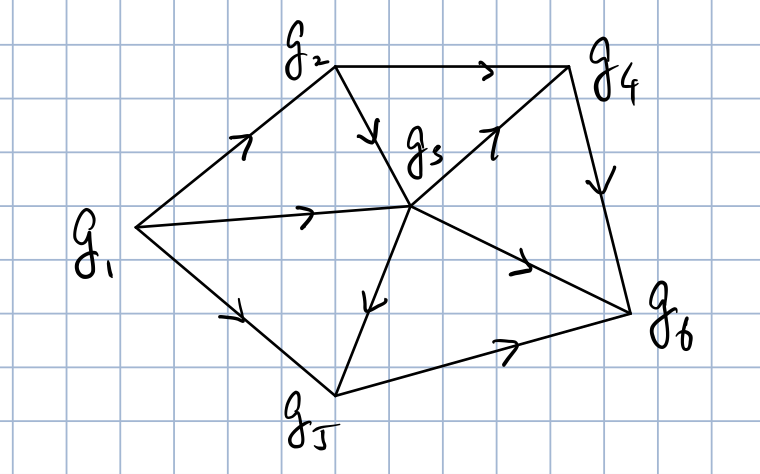
\includegraphics[height=3cm]{tri-lattice}
\end{center}
\end{frame}

\begin{frame}
\frametitle{Partition function}
\[Z = \sum_{\{g_i\}}e^{iS},\quad 
S = \sum_{\Delta ijk}2\pi s_{ijk}\omega(g_i,g_j,g_k).\]

\begin{center}
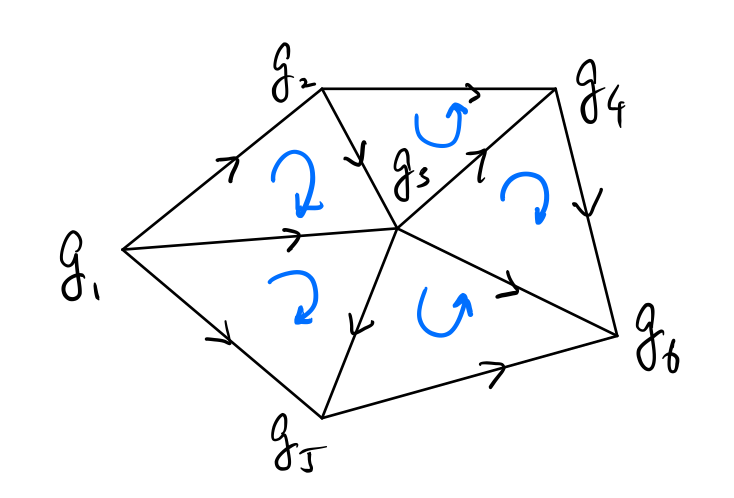
\includegraphics[height=4cm]{tri-orient}
\end{center}

Function $\omega:G\times G\times\cdots\times G\rightarrow \mathbb R/\mathbb Z$.
\end{frame}

\begin{frame}
\frametitle{Symmetry condition}

\begin{itemize}
\item $G$ action:
$\omega(g_1, \ldots, g_{d+1})\rightarrow \omega(gg_1, \ldots, gg_{d+1})$.
\item If $g$ is unitary: $S$ should be invariant. $\omega(g_1, \ldots, g_{d+1})= \omega(gg_1, \ldots, gg_{d+1})$.

\item $g$ is antiunitary: $S\rightarrow -S$. $\omega(g_1, \ldots, g_{d+1})= -\omega(gg_1, \ldots, gg_{d+1})$.
\item $s(g)=\pm1$ if g is unitary/antiunitary.
\item $G$-action on $\mathbb R/\mathbb Z$:
$g\cdot x=s(g)x$.
\item Homogeneous condition:
\[g\cdot\omega(g_1, \ldots, g_{d+1})= \omega(gg_1, \ldots, gg_{d+1})\]
\end{itemize}

\begin{center}
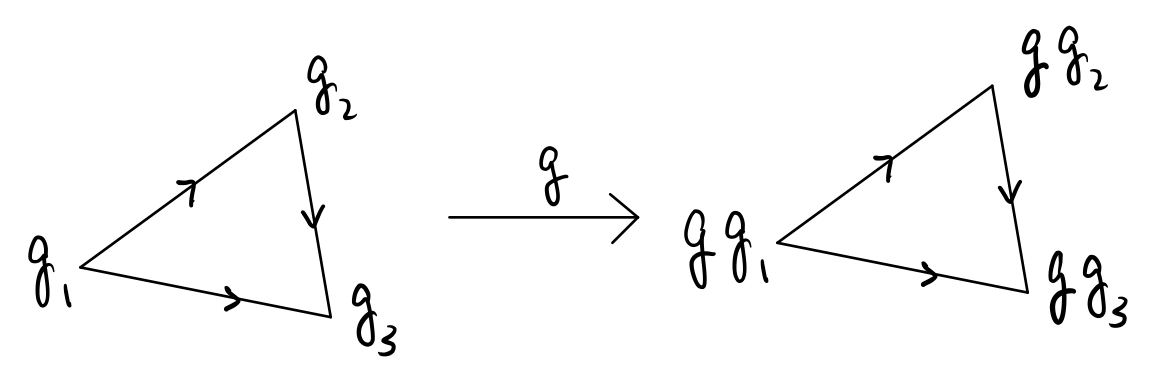
\includegraphics[height=2.5cm]{tri-action}
\end{center}
\end{frame}

\begin{frame}
\frametitle{Fixed-point properties: invariant under RG}
\begin{itemize}
\item SPT phases are gapped phases.
\item Gapped phases are stable fixed points in RG flow diagrams, with $\xi=0$.
\item Invariant under scale transformation.
\item Discrete version of scale transformation: re-triangularization.
\end{itemize}
\end{frame}

\begin{frame}
\frametitle{Cocycle conditions}
\end{frame}

\begin{frame}
\frametitle{Gauge transformation: coboundary equivalence}
\end{frame}

\begin{frame}
\frametitle{Formal definition: group cohomology}
\end{frame}

\section{Detecting an SPT state}

\begin{frame}
	\frametitle{Cannot detect from the bulk}
	\begin{itemize}
		\item Symmetry-breaking phases: detecting long-range order / Goldstone mode.
		\item SPT: Bulk is gapped and have trivial excitations.
		\item Edge states.
		\item Symmetry twist: Laughlin's argument.
	\end{itemize}
	\begin{center}
		%\includegraphics[height=4cm]{ti_band}
	\end{center}
\end{frame}

\section{Partition function and Group cohomology}

\begin{frame}
	\frametitle{Partition function of SPT state}
	\begin{itemize}
		\item Considier a finite, unitary symmetry group $G$.
		\item Use a cohomology class
		\[\alpha \in H^{d+1}[G, \uone].\]
		\item For a $(d+1)$-dimensional space-time manifold $M$,
		\item And $\gamma:\pi_1(M)\rightarrow G$,
		\[S_{\text{top}} = \langle \gamma^\ast\alpha,[M]\rangle.\]
	\end{itemize}
\end{frame}

\section{Standard resolution}

\begin{frame}
	\frametitle{Homogeneous cocycle}
	\begin{itemize}
		\item A homogeneous $k$-cocycle:
		\[\omega(g_0,\ldots,g_k)\in \uone.\]
		\item Coboundary:
		\[d\omega(g_0,\ldots,g_{k+1}) = \sum_{i=0}^{k+1}(-1)^i
		\omega(g_0,\ldots,\hat g_i,\ldots,g_{k+1}).\]
		\item Symmetry condition:
		\[\omega(gg_0,\ldots,gg_k)=\omega(g_0,\ldots,g_k)\]
		\item Lattice models on a $\Delta$-complex.
	\end{itemize}
\end{frame}

\end{document}
